\documentclass{minimal}
\usepackage{tikz}
\usetikzlibrary{external, calc, positioning,decorations.markings,arrows.meta}

%\tikzexternalize

\begin{document}
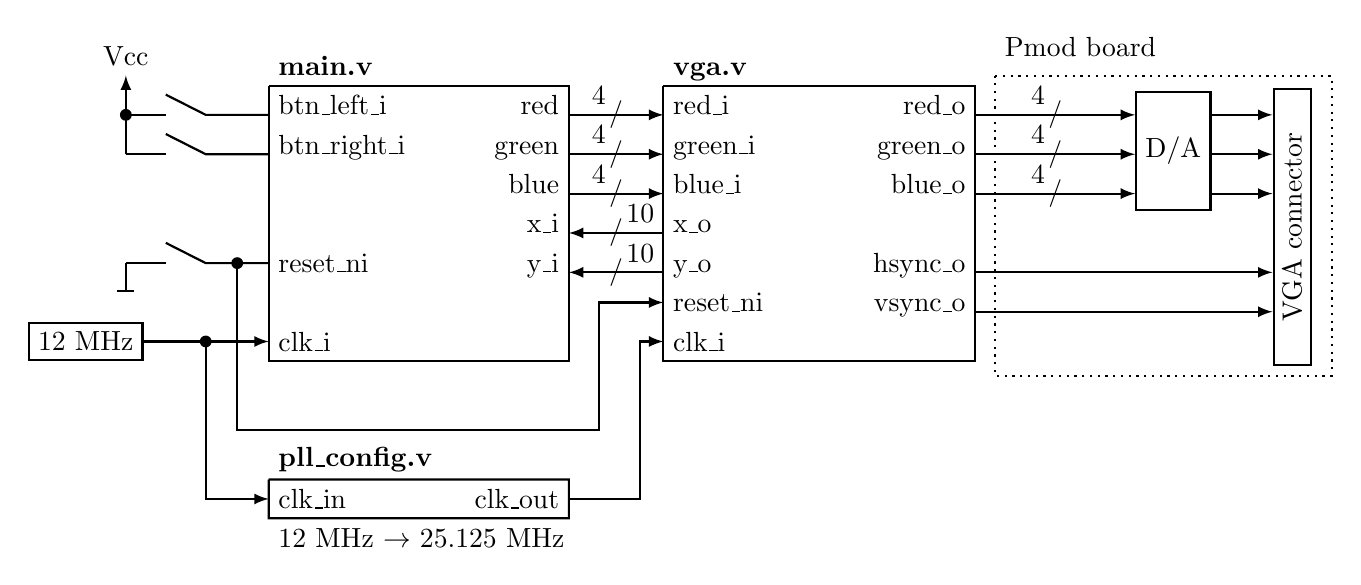
\begin{tikzpicture}[
	decoration={markings, 
	mark= at position 0.5 with {\node[]{/};}}
	]

		% main.v
		\node[anchor=west] (btnleft){btn\_left\_i};
		\node[below=5mm of btnleft.base west,anchor=base west] (btnright){btn\_right\_i};

		\node[below=15mm of btnright.base west,anchor=base west] (resetnim){reset\_ni};
		\node[below=10mm of resetnim.base west,anchor=base west] (clkinm){clk\_i};

		\node[right=30mm of btnleft.base,anchor=base east,align=right]
			(red){red};
		\node[below=5mm of red.base east,anchor=base east,align=right]
			(green){green};
		\node[below=5mm of green.base east,anchor=base east,align=right]
			(blue){blue};
		\node[below=5mm of blue.base east,anchor=base east,align=right]
			(xom){x\_i};
		\node[below=5mm of xom.base east,anchor=base east,align=right]
			(yom){y\_i};

		\draw[thick] (btnleft.north west)--(clkinm.south west)
			-- (clkinm.south west -| red.north east)
			-- (red.north east) -- (btnleft.north west);
		\node[above=5mm of btnleft.base west,anchor=base west](mainv){\textbf{main.v}};

		\node[left=8mm of btnleft.base west,anchor=base east,minimum height=5mm,minimum width=10mm](sw1){};
		\draw[thick] (btnleft.base west)--(sw1.east)--(sw1.north);
		\draw[thick] (sw1.center)--(sw1.west);
		\node[left=8mm of btnright.base west,anchor=base east,minimum height=5mm,minimum width=10mm](sw2){};
		\draw[thick] (btnright.base west)--(sw2.east)--(sw2.north);
		\draw[thick] (sw2.center)--(sw2.west);

		\draw[thick](sw2.west)--node[at end,circle,inner sep=0pt,minimum size=1.5mm,fill]{}(sw1.west);
		\node[above=5mm of sw1.west](vcc1){};
		\draw[thick,-latex](sw1.west)--node[at end,above]{Vcc}(vcc1);

		\node[thick,draw,left=25mm of clkinm.east,anchor=east](12mhz){12 MHz};
		\draw[thick,-latex](12mhz.east)--(clkinm.west);
		
		\node[left=8mm of resetnim.west,anchor=base east,minimum height=5mm,minimum width=10mm](sw3){};
		\node[below=25mm of vcc1.south,anchor=north](gnd1){};
		\draw[thick,-|](sw3)--(resetnim.west -| gnd1.north) -- (gnd1.south);
		\draw[thick] (resetnim.west)--node[fill,circle,inner sep=0pt,minimum size=1.5mm](ic3){}(sw3.east)--(sw3.north);
		\draw[thick] (sw3.center)--(sw3.west);

		\node[below=20mm of ic3.center](w1){};
		\node[below=25mm of sw3.east](w2){};
	
		% vga.v
		\node[right=12mm of red.base east,anchor=base west](redi){red\_i};
		\node[below=5mm of redi.base west,anchor=base west](greeni){green\_i};
		\node[below=5mm of greeni.base west,anchor=base west](bluei){blue\_i};

		\node[below=5mm of bluei.base west,anchor=base west](xo){x\_o};
		\node[below=5mm of xo.base west,anchor=base west](yo){y\_o};

		\node[below=20mm of greeni.base west,anchor=base west](resetniv){reset\_ni};
		\node[below=5mm of resetniv.base west,anchor=base west](clkiv){clk\_i};

		\node[right=30mm of redi.base east,anchor=base east,align=left](redo){red\_o};
		\node[below=5mm of redo.base east,anchor=base east,align=left](greeno){green\_o};
		\node[below=5mm of greeno.base east,anchor=base east,align=left](blueo){blue\_o};

		\node[below=10mm of blueo.base east,anchor=base east,align=left](hsynco){hsync\_o};
		\node[below=5mm of hsynco.base east,anchor=base east,align=left](vsynco){vsync\_o};

		\draw[thick] (redi.north west) -- (clkiv.south west) 
			-- (clkiv.south west -| redo.north east) -- (redo.north east)
			-- (redi.north west);
		\node[above=5mm of redi.base west,anchor=base west](vgav){\textbf{vga.v}};

		\draw[thick,-latex,postaction={decorate}](red.base east)-- node[above left](mid1){4}(redi.base west);
		\draw[thick,-latex,postaction={decorate}](green.base east)-- node[above left]{4}(greeni.base west);
		\draw[thick,-latex,postaction={decorate}](blue.base east)-- node[above left]{4}(bluei.base west);
		
		\draw[thick,latex-,postaction={decorate}](xom.base east)-- node[above right](mid2){10}(xo.base west);
		\draw[thick,latex-,postaction={decorate}](yom.base east)-- node[above right]{10}(yo.base west);

		\draw[thick,-latex](ic3.center)--(ic3.center |- w1) -- (w1 -| mid1.south) 
			-- (mid1.south |- resetniv.west) -- (resetniv.west);

		% pll_config.v
		\node[below=20mm of clkinm.base west,anchor=base west,align=left](pllclk){clk\_in};
		\node[below=30mm of yom.base east,anchor=base east,align=right](pxclk){clk\_out};
		\draw[thick,-latex](sw3.east |- 12mhz.east)node[circle,inner sep=0pt,minimum width=1.5mm,fill]{}
			--(pllclk.west -| w2)--(pllclk.west); 

		\draw[thick,-latex](pxclk.east)--(pxclk.east -| mid2) -- (mid2 |- clkiv.west)--(clkiv.west){};
		\draw[thick](pllclk.north west)--(pxclk.north east)--(pxclk.south east)--(pllclk.south west)
			--(pllclk.north west);

		\node[above=5mm of pllclk.west,anchor=west](pll){\textbf{pll\_config.v}};
		\node[below=5mm of pllclk.west,anchor=west]{12 MHz $\rightarrow$ 25.125 MHz};

		% PMOD	
		\node[right=30mm of greeno.east,anchor=east,minimum height=15mm,draw,thick](dac){D/A};
		\draw[thick,-latex,postaction={decorate}](redo.base east)--node[midway,above left]{4}
			(redo.base east -| dac.west);
		\draw[thick,-latex,postaction={decorate}](greeno.base east)--node[above left]{4}
			(greeno.base east -| dac.west);
		\draw[thick,-latex,postaction={decorate}](blueo.base east)--node[above left]{4}
			(blueo.base east -| dac.west);

		% VGA connector
		\node[right=70mm of xo.east,draw,thick,minimum height=35mm](con){\rotatebox{90}{VGA connector}};
		\draw[thick,-latex](dac.east |- redo.base east) -- (redo.base east -| con.west);
		\draw[thick,-latex](dac.east |- greeno.base east) -- (greeno.base east -| con.west);
		\draw[thick,-latex](dac.east |- blueo.base east) -- (blueo.base east -| con.west);
		
		\draw[thick,-latex](hsynco.base east) -- (hsynco.base east -| con.west);
		\draw[thick,-latex](vsynco.base east) -- (vsynco.base east -| con.west);

		% PMOD dotted
		\node[right=5mm of redo.north east,anchor=base east](pmod1){};
		\node[right=0mm of con.south east](pmod2){};
		\draw[thick,dotted] (pmod1.north west)--(pmod1.north west -| pmod2.south east) 
			-- (pmod2.south east) -- (pmod2.south east -| pmod1.north west) -- (pmod1.north west);
		\node[above=5mm of pmod1.west,anchor=west](){Pmod board};

	\end{tikzpicture}
\end{document}
